\section{Datasets}
\label{app:datasets}

\subsection{Dataset statistics}
First, \autoref{tab:app_datasets_transd}, \autoref{tab:app_datasets_inde}, and \autoref{tab:app_datasets_indr} provide the necessary details on the graphs behind the \clqa datasets. 
Then, \autoref{tab:app_transd_queries}, \autoref{tab:app_inductive_e_queries}, and \autoref{tab:wikitopics-clqa} list the query statistics. 
Transductive datasets are BetaE~\citep{betae} datasets (MIT license), inductive $(e)$ datasets are adopted from \citet{galkin2022} (CC BY 4.0 license) where validation and test inference graphs extend the training graph. The ratio denotes the size of the inference graph to the size of the training graph (in the number of nodes), that is, $\gV_{\textit{inf}} / \gV_{\textit{train}}$.
In the following \Cref{app:subsec_wikitopcs_clqa} we provide more details in sampling 11 new inductive $(e,r)$ datasets WikiTopics-CLQA (available under the CC BY 4.0 license).


\begin{table}[!ht]
\centering
\caption{Graph in transductive datasets (3) from \citet{betae}. Inverse triples and edge types are included in the splits. Train, Valid, Test denote triples in the respective set. }
\label{tab:app_datasets_transd}
%\scriptsize
%\begin{adjustbox}{width=\textwidth}
\begin{tabular}{lccccc}\toprule
Dataset &Entities &Rels &Train &Valid &Test  \\\midrule
FB15k & 14,951 & 2,690 & 966,284 & 100,000 & 118,142 \\
FB15k237 &14,505 &474 &544,230 &35,052 &40,876 \\
NELL995  &63,361 &400 &228,426 &28,648 & 28,534 \\
\bottomrule
\end{tabular}
%\end{adjustbox}
%
\caption{Graphs in inductive $(e)$ datasets (9) from \citet{galkin2022}. Inverse triples and edge types are included in all graphs. Validation and Test splits contain an inference graph $(\gV_\textit{inf}, \gE_\textit{inf})$ which is a superset of the training graph with new nodes, and missing edges to predict (Valid and Test, respectively).  }
\label{tab:app_datasets_inde}
%\scriptsize
\begin{adjustbox}{width=\textwidth}
\begin{tabular}{ccccccccccc}\toprule
\multirow{2}{*}{Ratio, \%} &\multirow{2}{*}{Rels} &\multicolumn{2}{c}{Training Graph} &\multicolumn{3}{c}{Validation Graph} &\multicolumn{3}{c}{Test Graph} \\ \cmidrule(lr){3-4}  \cmidrule(lr){5-7}  \cmidrule(lr){8-10}
& &Entities & Triples & Entities & Triples & Valid & Entities & Triples & Test \\ \midrule
106\% &466 &13,091 &493,425 &13,801 &551,336 &10,219 &13,802 &538,896 &8,023 \\
113\% &468 &11,601 &401,677 &13,022 &491,518 &15,849 &13,021 &486,068 &14,893 \\
122\% &466 &10,184 &298,879 &12,314 &413,554 &20,231 &12,314 &430,892 &23,289 \\
134\% &466 &8,634 &228,729 &11,468 &373,262 &25,477 &11,471 &367,810 &24,529 \\
150\% &462 &7,232 &162,683 &10,783 &311,462 &26,235 &10,782 &331,352 &29,755 \\
175\% &436  &5,560 &102,521 &9,801 &265,412 &28,691 &9,781 &266,494 &28,891 \\
217\% &446  &4,134 &52,455 &9,062 &227,284 &30,809 &9,058 &212,386 &28,177 \\
300\% &412  &2,650 &24,439 &8,252 &178,680 &27,135 &8,266 &187,156 &28,657 \\
550\% &312  &1,084 &5,265 &7,247 &136,558 &22,981 &7,275 &133,524 &22,503 \\
\bottomrule
\end{tabular}
\end{adjustbox}
\caption{Graphs in the newly sampled inductive entity and relation $(e,r)$ WikiTopics-CLQA datasets (11). Triples denote the number of edges of the graph given at training, validation, or test. Valid and Test denote triples to be predicted in the validation and test sets in the respective validation and test graph. 
% In accordance with the setting of WikiTopics~\cite{isdea}, the validation graph is a superset of the training graph, but the test graph is a 
}
\label{tab:app_datasets_indr}
%\scriptsize
\begin{adjustbox}{width=\textwidth}
\begin{tabular}{lcccccccccccc}\toprule
\multirow{2}{*}{Dataset} &\multicolumn{3}{c}{Training Graph} &\multicolumn{4}{c}{Validation Graph} &\multicolumn{4}{c}{Test Graph} \\ \cmidrule(l){2-4} \cmidrule(l){5-8} \cmidrule(l){9-12}
&Entities &Rels &Triples &Entities &Rels &Triples &Valid &Entities &Rels &Triples &Test \\\midrule
Art &10000 &65 &27262 &10000 &65 &27262 &3026 &10000 &65 &28023 &3113 \\
Award &10000 &17 &23821 &10000 &13 &23821 &2646 &10000 &17 &25056 &2783 \\
Education &10000 &19 &14355 &10000 &19 &14355 &1594 &10000 &19 &14193 &1575 \\
Health &10000 &31 &15539 &10000 &31 &15539 &1725 &10000 &31 &15337 &1703 \\
Infrastructure &10000 &37 &21990 &10000 &37 &21990 &2443 &10000 &37 &21646 &2405 \\
Location &10000 &62 &85063 &10000 &62 &85063 &9451 &10000 &62 &80269 &8917 \\
Organization &10000 &34 &33325 &10000 &34 &33325 &3702 &10000 &34 &31314 &3357 \\
People &10000 &40 &55698 &10000 &40 &55698 &6188 &10000 &40 &58530 &6503 \\
Science &10000 &66 &12576 &10000 &66 &12576 &1397 &10000 &66 &12516 &1388 \\
Sport &10000 &34 &47251 &10000 &34 &47251 &5250 &10000 &34 &46717 &5190 \\
Taxonomy &10000 &59 &18921 &10000 &59 &18921 &2102 &10000 &59 &19416 &2157 \\
\bottomrule
\end{tabular}
\end{adjustbox}
\end{table}


%%% TODO: Dataset statistics table
\begin{table}[!ht]
\centering
    \caption{Statistics of 3 transductive datasets}
    \begin{adjustbox}{max width=0.48\textwidth}
        \begin{tabular}{llcccc}
            \toprule
            \bf{Split} & \bf{Query Type} & \bf{FB15k} & \bf{FB15k-237} & \bf{NELL995} \\
            \midrule
            \multirow{2}{*}{Train}
            & 1p/2p/3p/2i/3i & 273,710 & 149,689 & 107,982 \\
            & 2in/3in/inp/pin/pni & 27,371 & 14,968 & 10,798 \\
            \midrule
            \multirow{2}{*}{Valid}
            & 1p & 59,078 & 20,094 & 16,910 \\
            & Others & 8,000 & 5,000 & 4,000 \\
            \midrule
            \multirow{2}{*}{Test}
            & 1p & 66,990 & 22,804 & 17,021 \\
            & Others & 8,000 & 5,000 & 4,000 \\
            \bottomrule
        \end{tabular}
    \end{adjustbox}
    \label{tab:app_transd_queries}
%
\centering
\caption{Statistics of 9 inductive $(e)$ datasets.}
\label{tab:app_inductive_e_queries}
%\scriptsize
\begin{adjustbox}{width=\textwidth}
\begin{tabular}{lrrrrrrrrrrrrrrrr}\toprule
Ratio & Graph & \multicolumn{1}{c}{\textbf{1p}} & \multicolumn{1}{c}{\textbf{2p}} & \multicolumn{1}{c}{\textbf{3p}} & \multicolumn{1}{c}{\textbf{2i}} & \multicolumn{1}{c}{\textbf{3i}} & \multicolumn{1}{c}{\textbf{pi}} & \multicolumn{1}{c}{\textbf{ip}} & \multicolumn{1}{c}{\textbf{2u}} & \multicolumn{1}{c}{\textbf{up}} & \multicolumn{1}{c}{\textbf{2in}} & \multicolumn{1}{c}{\textbf{3in}} & \multicolumn{1}{c}{\textbf{inp}} & \multicolumn{1}{c}{\textbf{pin}} & \multicolumn{1}{c}{\textbf{pni}} \\\midrule
\multirow{3}{*}{106\%} &training & 135,613 &50,000 &50,000 &50,000 &50,000 &50,000 &50,000 &50,000 &50,000 &50,000 &40,000 &50,000 &50,000 &50,000 \\
&validation & 6,582 &10,000 &10,000 &10,000 &10,000 &10,000 &10,000 &10,000 &10,000 &1,000 &1,000 &1,000 &1,000 &1,000 \\
&test & 5,446 &10,000 &10,000 &10,000 &10,000 &10,000 &10,000 &10,000 &10,000 &1,000 &1,000 &1,000 &1,000 &1,000 \\ \midrule
\multirow{3}{*}{113\%} &training & 115,523 &50,000 &50,000 &50,000 &50,000 &50,000 &50,000 &50,000 &50,000 &50,000 &40,000 &50,000 &50,000 &50,000 \\
&validation & 10,256 &10,000 &10,000 &10,000 &10,000 &10,000 &10,000 &10,000 &10,000 &1,000 &1,000 &1,000 &1,000 &1,000 \\
&test & 9,782 &10,000 &10,000 &10,000 &10,000 &10,000 &10,000 &10,000 &10,000 &1,000 &1,000 &1,000 &1,000 &1,000 \\ \midrule
\multirow{3}{*}{121\%} &training & 91,228 &50,000 &50,000 &50,000 &50,000 &50,000 &50,000 &50,000 &50,000 &50,000 &40,000 &50,000 &50,000 &50,000 \\
&validation & 12,696 &10,000 &10,000 &10,000 &10,000 &10,000 &10,000 &10,000 &10,000 &5,000 &5,000 &5,000 &5,000 &5,000 \\
&test & 14,458 &10,000 &10,000 &10,000 &10,000 &10,000 &10,000 &10,000 &10,000 &5,000 &5,000 &5,000 &5,000 &5,000 \\ \midrule
\multirow{3}{*}{133\%} &training & 75,326 &50,000 &50,000 &50,000 &50,000 &50,000 &50,000 &50,000 &50,000 &50,000 &40,000 &50,000 &50,000 &50,000 \\
&validation & 15,541 &50,000 &50,000 &50,000 &50,000 &50,000 &50,000 &20,000 &20,000 &5,000 &5,000 &5,000 &5,000 &5,000 \\
&test & 15,270 &50,000 &50,000 &50,000 &50,000 &50,000 &50,000 &20,000 &20,000 &5,000 &5,000 &5,000 &5,000 &5,000 \\ \midrule
\multirow{3}{*}{150\%} &training & 56,114 &50,000 &50,000 &50,000 &50,000 &50,000 &50,000 &50,000 &50,000 &50,000 &40,000 &50,000 &50,000 &50,000 \\
&validation & 16,229 &50,000 &50,000 &50,000 &50,000 &50,000 &50,000 &50,000 &50,000 &5,000 &5,000 &5,000 &5,000 &5,000 \\
&test & 17,683 &50,000 &50,000 &50,000 &50,000 &50,000 &50,000 &50,000 &50,000 &5,000 &5,000 &5,000 &5,000 &5,000 \\ \midrule
\multirow{3}{*}{175\%} &training & 38,851 &50,000 &50,000 &50,000 &50,000 &50,000 &50,000 &50,000 &50,000 &50,000 &40,000 &50,000 &50,000 &50,000 \\
&validation & 17,235 &50,000 &50,000 &50,000 &50,000 &50,000 &50,000 &50,000 &50,000 &10,000 &10,000 &10,000 &10,000 &10,000 \\
&test & 17,476 &50,000 &50,000 &50,000 &50,000 &50,000 &50,000 &50,000 &50,000 &10,000 &10,000 &10,000 &10,000 &10,000 \\ \midrule
\multirow{3}{*}{217\%} & training & 22,422 &30,000 &30,000 &50,000 &50,000 &50,000 &50,000 &50,000 &50,000 &30,000 &30,000 &50,000 &50,000 &50,000 \\
&validation & 18,168 &50,000 &50,000 &50,000 &50,000 &50,000 &50,000 &50,000 &50,000 &10,000 &10,000 &10,000 &10,000 &10,000 \\
&test & 16,902 &50,000 &50,000 &50,000 &50,000 &50,000 &50,000 &50,000 &50,000 &10,000 &10,000 &10,000 &10,000 &10,000 \\ \midrule
\multirow{3}{*}{300\%} &training & 11,699 &15,000 &15,000 &40,000 &40,000 &50,000 &50,000 &50,000 &50,000 &15,000 &15,000 &50,000 &40,000 &50,000 \\
&validation & 16,189 &50,000 &50,000 &50,000 &50,000 &50,000 &50,000 &50,000 &50,000 &10,000 &10,000 &10,000 &10,000 &10,000 \\
&test & 17,105 &50,000 &50,000 &50,000 &50,000 &50,000 &50,000 &50,000 &50,000 &10,000 &10,000 &10,000 &10,000 &10,000 \\ \midrule
\multirow{3}{*}{550\%} &training & 3,284 &15,000 &15,000 &40,000 &40,000 &50,000 &50,000 &50,000 &50,000 &10,000 &10,000 &30,000 &30,000 &30,000 \\
&validation & 13,616 &50,000 &50,000 &50,000 &50,000 &50,000 &50,000 &50,000 &50,000 &10,000 &10,000 &10,000 &10,000 &10,000 \\
&test & 13,670 &50,000 &50,000 &50,000 &50,000 &50,000 &50,000 &50,000 &50,000 &10,000 &10,000 &10,000 &10,000 &10,000 \\ 
\bottomrule
\end{tabular}
\end{adjustbox}
%
\centering
\caption{WikiTopics-CLQA statistics: the number of queries generated per query pattern for each topic knowledge graph of WikiTopics~\citep{isdea}. Numbers are the same for both the training and inference graph.  We follow the same 14 query patterns introduced by~\citet{betae}.}
%\scriptsize
\begin{adjustbox}{width=\textwidth}
\begin{tabular}{lrrrrrrrrrrrrrrr}\toprule
Topics & \bf{1p} & \bf{2p} & \bf{3p} & \bf{2i} & \bf{3i} & \bf{pi} & \bf{ip} & \bf{2in} & \bf{3in} & \bf{pin} & \bf{pni} & \bf{inp} & \bf{2u} & \bf{up} \\
\midrule
Art & 3113 & 10000 & 10000 & 10000 & 10000 & 10000 & 10000 & 1000 & 1000 & 1000 & 1000 & 1000 & 10000 & 10000 \\
Award & 2783 & 10000 & 10000 & 10000 & 10000 & 10000 & 10000 & 1000 & 1000 & 1000 & 1000 & 1000 & 10000 & 10000 \\
Education & 1575 & 10000 & 10000 & 10000 & 10000 & 10000 & 10000 & 1000 & 1000 & 1000 & 1000 & 1000 & 10000 & 10000 \\
Health & 1703 & 10000 & 10000 & 10000 & 10000 & 10000 & 10000 & 1000 & 1000 & 1000 & 1000 & 1000 & 10000 & 10000 \\
Infrastructure & 2405 & 10000 & 10000 & 10000 & 10000 & 10000 & 10000 & 1000 & 1000 & 1000 & 1000 & 1000 & 10000 & 10000 \\
Location & 8000 & 8917 & 4000 & 8000 & 8000 & 8000 & 8000 & 1000 & 1000 & 1000 & 1000 & 1000 & 8000 & 8000 \\
Organization & 3357 & 8000 & 4000 & 8000 & 8000 & 8000 & 8000 & 1000 & 1000 & 1000 & 1000 & 1000 & 8000 & 8000 \\
People & 6503 & 10000 & 10000 & 10000 & 10000 & 10000 & 10000 & 1000 & 1000 & 1000 & 1000 & 1000 & 10000 & 10000 \\
Science & 1388 & 10000 & 10000 & 10000 & 10000 & 10000 & 10000 & 1000 & 1000 & 1000 & 1000 & 1000 & 10000 & 10000 \\
Sport & 5190 & 8000 & 4000 & 8000 & 8000 & 8000 & 8000 & 1000 & 1000 & 1000 & 1000 & 1000 & 8000 & 8000 \\
Taxonomy & 2157 & 8000 & 8000 & 8000 & 8000 & 8000 & 8000 & 1000 & 1000 & 1000 & 1000 & 1000 & 8000 & 8000 \\
\bottomrule
\end{tabular}
\end{adjustbox}
\label{tab:wikitopics-clqa}
\end{table}

\subsection{WikiTopics-CLQA}
\label{app:subsec_wikitopcs_clqa}

The WikiTopics dataset introduced by~\citet{isdea} was used to evaluate link prediction model's zero-shot performance in the  inductive $(e,r)$ setting, i.e., when the test-time inference graph contains \textit{both} new entities and new relations unseen in training. It grouped relations into 11 different topics, or domains, such as art, education, health care, and sport. Two graphs, $\gtrain^{(T)}$ and $\ginf^{(T)}$ along with the missing triples $\edges^{(T)}_{\textit{valid}}$ and $\edges^{(T)}_{\textit{test}}$, were provided for each topic $T$, which had the same set of relations but different (potentially overlapping) set of entities. 
The goal was to train models on the training graphs $\gtrain^{(T)}$ of some topic $T$, and test on the inference graph $\ginf^{(T')}$ of an unseen topic $T'$. 
The model's validation performance was evaluated on the missing triples $\edges^{(T)}_{\textit{valid}}$ when observing training graph $\gtrain^{(T)}$ as inputs, and its test performance was evaluated on $\edges^{(T')}_{\textit{test}}$ when observing the test inference graph $\ginf^{(T')}$ as inputs. \Cref{tab:app_datasets_indr} shows the statistics of the 11 topic-specific knowledge graphs in WikiTopics.

We follow the procedures in BetaE~\citep{betae} to generate queries and answers of the 14 query patterns using the knowledge graphs in WikiTopics. We name the resulting dataset WikiTopics-CLQA. 
% We generate queries and answers for the training graph $\gtrain^{(T)}$ and inference graph $\ginf^{(T)}$ separately for each topic $T$
% , and we treat the label split, $\gG_{\textit{train-label}}^{(T)}$ and $\gG_{\textit{inf-label}}^{(T)}$, as the missing links, from which we extract the \textit{hard} answers. That is, entities that cannot be achieved by traversing the graph unless the missing link is predicted. 
For each topic $T$, we generate three sets of queries and answers (training, validation, test), using the training graph $\gtrain^{(T)}$ for training and validation, and inference graph $\ginf^{(T)}$ for test queries, respectively. 
Training queries on $\gtrain^{(T)}$ only have easy answers, 
validation (test) set easy answers are attained by traversing  $\gtrain^{(T)}$ ($\ginf^{(T)}$), whereas the full set of answers (easy and hard) are attained by traversing the graph $\gtrain^{(T)}$ merged with $\edges^{(T)}_{\textit{valid}}$ ($\ginf^{(T)}$ merged with $\edges^{(T)}_{\textit{test}}$). Hence, the hard answers cannot be found unless the model is capable of imputing missing links.
In our experiments, we only use the inference graph $\ginf^{(T)}$ and the test queries and answers for evaluating zero-shot inference performance.
%
\Cref{tab:wikitopics-clqa} shows the statistics of the WikiTopics-CLQA dataset. 

\section{Hyperparameters and Baselines}
\label{app:hyperparams}

Both \method and \methodlp are implemented with PyTorch~\cite{pytorch} (BSD-style license) and PyTorch-Geometric~\cite{pyg} (MIT license).
Both \method and \methodlp are initialized from the pre-trained \ultra checkpoint published by the authors and have the same GNN architectures with parameter count (177k).
\method is further trained for 10,000 steps on complex queries from the FB15k237 dataset. 
Hyperparameters of \method and its training details are listed in \autoref{tab:ultraquery_hparams}.

\methodlp employs thresholding of intermediate fuzzy set scores as one of the ways to alleviate the multi-source propagation issue (\Cref{subsec:ultra_proj}). 
Generally, the threshold is set to 0.8 with a few exceptions:
\begin{itemize}[leftmargin=*]
    \item 0.97 in NELL995
\end{itemize}

Below, we discuss the best available baselines for each dataset family.

\textbf{Transductive} (3 datasets): QTO~\citep{qto}. QTO requires  2000$d$ ComplEx~\citep{complex} entity and relation embeddings pre-computed for each graph, \eg, taking 30M parameters on the FB15k237 graph with 15k nodes. 
Further, QTO materializes the whole $(\gV \times \gV \times \gR)$ 3D tensor of scores of all possible triples for each graph. 
Pre-computing such tensors on three datasets takes considerable space and time, \eg, 8 hours for FB15k with heavy sparsification settings to fit onto a 24 GB GPU.

\textbf{Inductive $(e)$} (9 datasets): GNN-QE~\citep{gnn_qe}. The framework of GNN-QE is similar to \method but the backbone relation projection operator is implemented with NBFNet~\citep{nbfnet} which is only inductive to entities and still learns graph-specific relation embeddings. 
Parameter count, therefore, depends on the number of unique relation types, \eg, 2M for the FB 175\% split with 436 unique relations.

\textbf{Inductive $(e,r)$} (11 datasets): for newly sampled datasets, due to the absence of fully inductive trainable baselines, we compare against a rule-based heuristic baseline similar to the baseline in \citet{galkin2022}.
The baseline looks up candidate entities that have the same incoming relation type as the current relation projection (note that the identity of the starting head node in this case is ignored). 
The heuristic filters entities into two classes (satisfying the incoming relation type or not), hence, in order to create a ranking, we randomly shuffle entities in each class.
This baseline is non-parametric, does not require any training, and represents a sanity check of \clqa models. Still, as shown in \citet{galkin2022}, the baseline might outperform certain inductive reasoning approaches parameterized by neural networks. 


\begin{table}[t]
\centering
\caption{\method hyperparameters. $\text{GNN}_r$ denotes a GNN over the graph of relations $\grel$, $\text{GNN}_e$ is a GNN over the original entity graph $\gG$.}
\label{tab:ultraquery_hparams}
%\scriptsize
\begin{tabular}{lccc}\toprule
\multicolumn{2}{l}{Hyperparameter} &\method training \\\midrule
\multirow{4}{*}{$\text{GNN}_r$} &\# layers &6 \\
&hidden dim &64 \\
&message &DistMult \\
&aggeregation &sum \\ \midrule
\multirow{5}{*}{$\text{GNN}_e$} &\# layers &6 \\
&hidden dim &64 \\
&message &DistMult \\
&aggregation &sum \\
&$g(\cdot)$ &2-layer MLP \\ \midrule
\multirow{7}{*}{Learning} &optimizer &AdamW \\
&learning rate &0.0005 \\
&training steps &10,000 \\
&adv temperature & 0.2 \\
&traversal dropout & 0.25 \\
&batch size &64 \\
&training queries &FB15k237 \\
\bottomrule
\end{tabular}
\end{table}

\section{More Results}
\label{app:more_results}

\autoref{tab:app_full_results} corresponds to \autoref{fig:main_fig1} and \autoref{tab:maintab1} and provides MRR and Hits@10 results for \method, \methodlp, and Best Baseline for each dataset averaged across 9 EPFO query types and 5 negation query types. 
\autoref{fig:app_inde_full} is the full version of \autoref{fig:abl_multisource} and illustrates the performance of all 3 compared models on 9 inductive $(e)$ datasets on 14 query types together with their averaged values (EPFO avg and neg avg, respectively).

%%% ULTRA-Query More Results %%%
\begin{table}[!ht]
\centering
\caption{Full results (MRR, Hits@10) of \methodlp and \method in the zero-shot inference regime on transductive, entity-inductive $(e)$, and fully inductive $(e, r)$ datasets compared to the best-reported baselines averaged across 9 EPFO query types (EPFO avg) and 5 negation query types (Negation avg). \method was fine-tuned only on FB15k237 queries. The numbers correspond to~\Cref{tab:maintab1} and \Cref{fig:main_fig1}.}
\label{tab:app_full_results}
\begin{adjustbox}{width=\textwidth}
\begin{tabular}{lcccccccccccc}\toprule
&\multicolumn{4}{c}{\bf{\methodlp}} &\multicolumn{4}{c}{\bf{\method}} &\multicolumn{4}{c}{\bf{Best Baseline}}  \\  \cmidrule(l){2-5} \cmidrule(l){6-9} \cmidrule(l){10-13}
&\multicolumn{2}{c}{\bf{EPFO avg}} &\multicolumn{2}{c}{\bf{Negation avg}} &\multicolumn{2}{c}{\bf{EPFO avg}} &\multicolumn{2}{c}{\bf{Negation avg}} &\multicolumn{2}{c}{\bf{EPFO avg}} &\multicolumn{2}{c}{\bf{Negation avg}} \\ \cmidrule(l){2-3} \cmidrule(l){2-3} \cmidrule(l){4-5}  \cmidrule(l){6-7} \cmidrule(l){8-9} \cmidrule(l){10-11} \cmidrule(l){12-13} 
&MRR &Hits@10 &MRR &Hits@10  &MRR &Hits@10  &MRR &Hits@10  &MRR &Hits@10  &MRR &Hits@10 \\ \midrule
\multicolumn{13}{c}{transductive datasets} \\ \midrule
FB15k237 &0.216 &0.362 &0.082 &0.164 &0.242 &0.378 &0.08 &0.174 &0.335 &0.491 &0.155 &0.295 \\
FB15k &0.501 &0.672 &0.291 &0.465 &0.764 &0.834 &0.567 &0.725 &0.74 &0.837 &0.492 &0.664 \\
NELL995 &0.249 &0.395 &0.079 &0.16 &0.226 &0.341 &0.073 &0.159 &0.329 &0.483 &0.129 &0.268 \\ \midrule
\multicolumn{13}{c}{inductive $(e)$ datasets} \\ \midrule
FB 550\% &0.340 &0.518 &0.134 &0.251 &0.373 &0.535 &0.186 &0.332 &0.222 &0.331 &0.091 &0.158 \\
FB 300\% &0.320 &0.496 &0.117 &0.227 &0.359 &0.526 &0.168 &0.312 &0.291 &0.426 &0.125 &0.224 \\
FB 217\% &0.332 &0.509 &0.133 &0.252 &0.375 &0.537 &0.186 &0.337 &0.346 &0.492 &0.174 &0.301 \\
FB 175\% &0.297 &0.469 &0.110 &0.214 &0.338 &0.499 &0.159 &0.297 &0.351 &0.507 &0.188 &0.336 \\
FB 150\% &0.279 &0.445 &0.097 &0.190 &0.316 &0.473 &0.132 &0.255 &0.339 &0.493 &0.167 &0.303 \\
FB 133\% &0.266 &0.426 &0.087 &0.167 &0.298 &0.451 &0.122 &0.238 &0.353 &0.514 &0.197 &0.341 \\
FB 121\% &0.246 &0.400 &0.081 &0.164 &0.279 &0.430 &0.119 &0.232 &0.323 &0.462 &0.173 &0.291 \\
FB 113\% &0.217 &0.362 &0.067 &0.136 &0.240 &0.387 &0.097 &0.192 &0.352 &0.494 &0.214 &0.339 \\
FB 106\% &0.200 &0.340 &0.054 &0.114 &0.226 &0.370 &0.086 &0.162 &0.373 &0.504 &0.256 &0.377 \\ \midrule
\multicolumn{13}{c}{inductive $(e, r)$ datasets} \\ \midrule
Art &0.249 &0.389 &0.086 &0.157 &0.248 &0.349 &0.083 &0.137 &0.016 &0.031 &0.006 &0.014 \\
Award &0.224 &0.413 &0.046 &0.098 &0.227 &0.354 &0.152 &0.274 &0.004 &0.006 &0.002 &0.002 \\
Edu &0.142 &0.258 &0.066 &0.122 &0.179 &0.249 &0.119 &0.176 &0.008 &0.014 &0.003 &0.005 \\
Health &0.317 &0.466 &0.159 &0.231 &0.317 &0.394 &0.419 &0.525 &0.019 &0.040 &0.010 &0.020 \\
Infrastructure &0.392 &0.551 &0.087 &0.170 &0.337 &0.461 &0.235 &0.356 &0.010 &0.018 &0.003 &0.005 \\
Location &0.508 &0.678 &0.198 &0.371 &0.569 &0.679 &0.402 &0.585 &0.007 &0.017 &0.001 &0.002 \\
Organization &0.098 &0.190 &0.023 &0.048 &0.169 &0.270 &0.082 &0.171 &0.005 &0.008 &0.001 &0.002 \\
People &0.373 &0.530 &0.182 &0.281 &0.332 &0.443 &0.194 &0.285 &0.005 &0.010 &0.002 &0.003 \\
Science &0.206 &0.348 &0.048 &0.093 &0.158 &0.255 &0.071 &0.131 &0.041 &0.085 &0.010 &0.020 \\
Sport &0.215 &0.357 &0.095 &0.166 &0.252 &0.371 &0.178 &0.269 &0.015 &0.030 &0.005 &0.008 \\
Taxonomy &0.230 &0.315 &0.151 &0.255 &0.290 &0.360 &0.183 &0.261 &0.034 &0.066 &0.009 &0.017 \\
\bottomrule
\end{tabular}
\end{adjustbox}
\end{table}

\begin{figure*}[t]
    \centering
    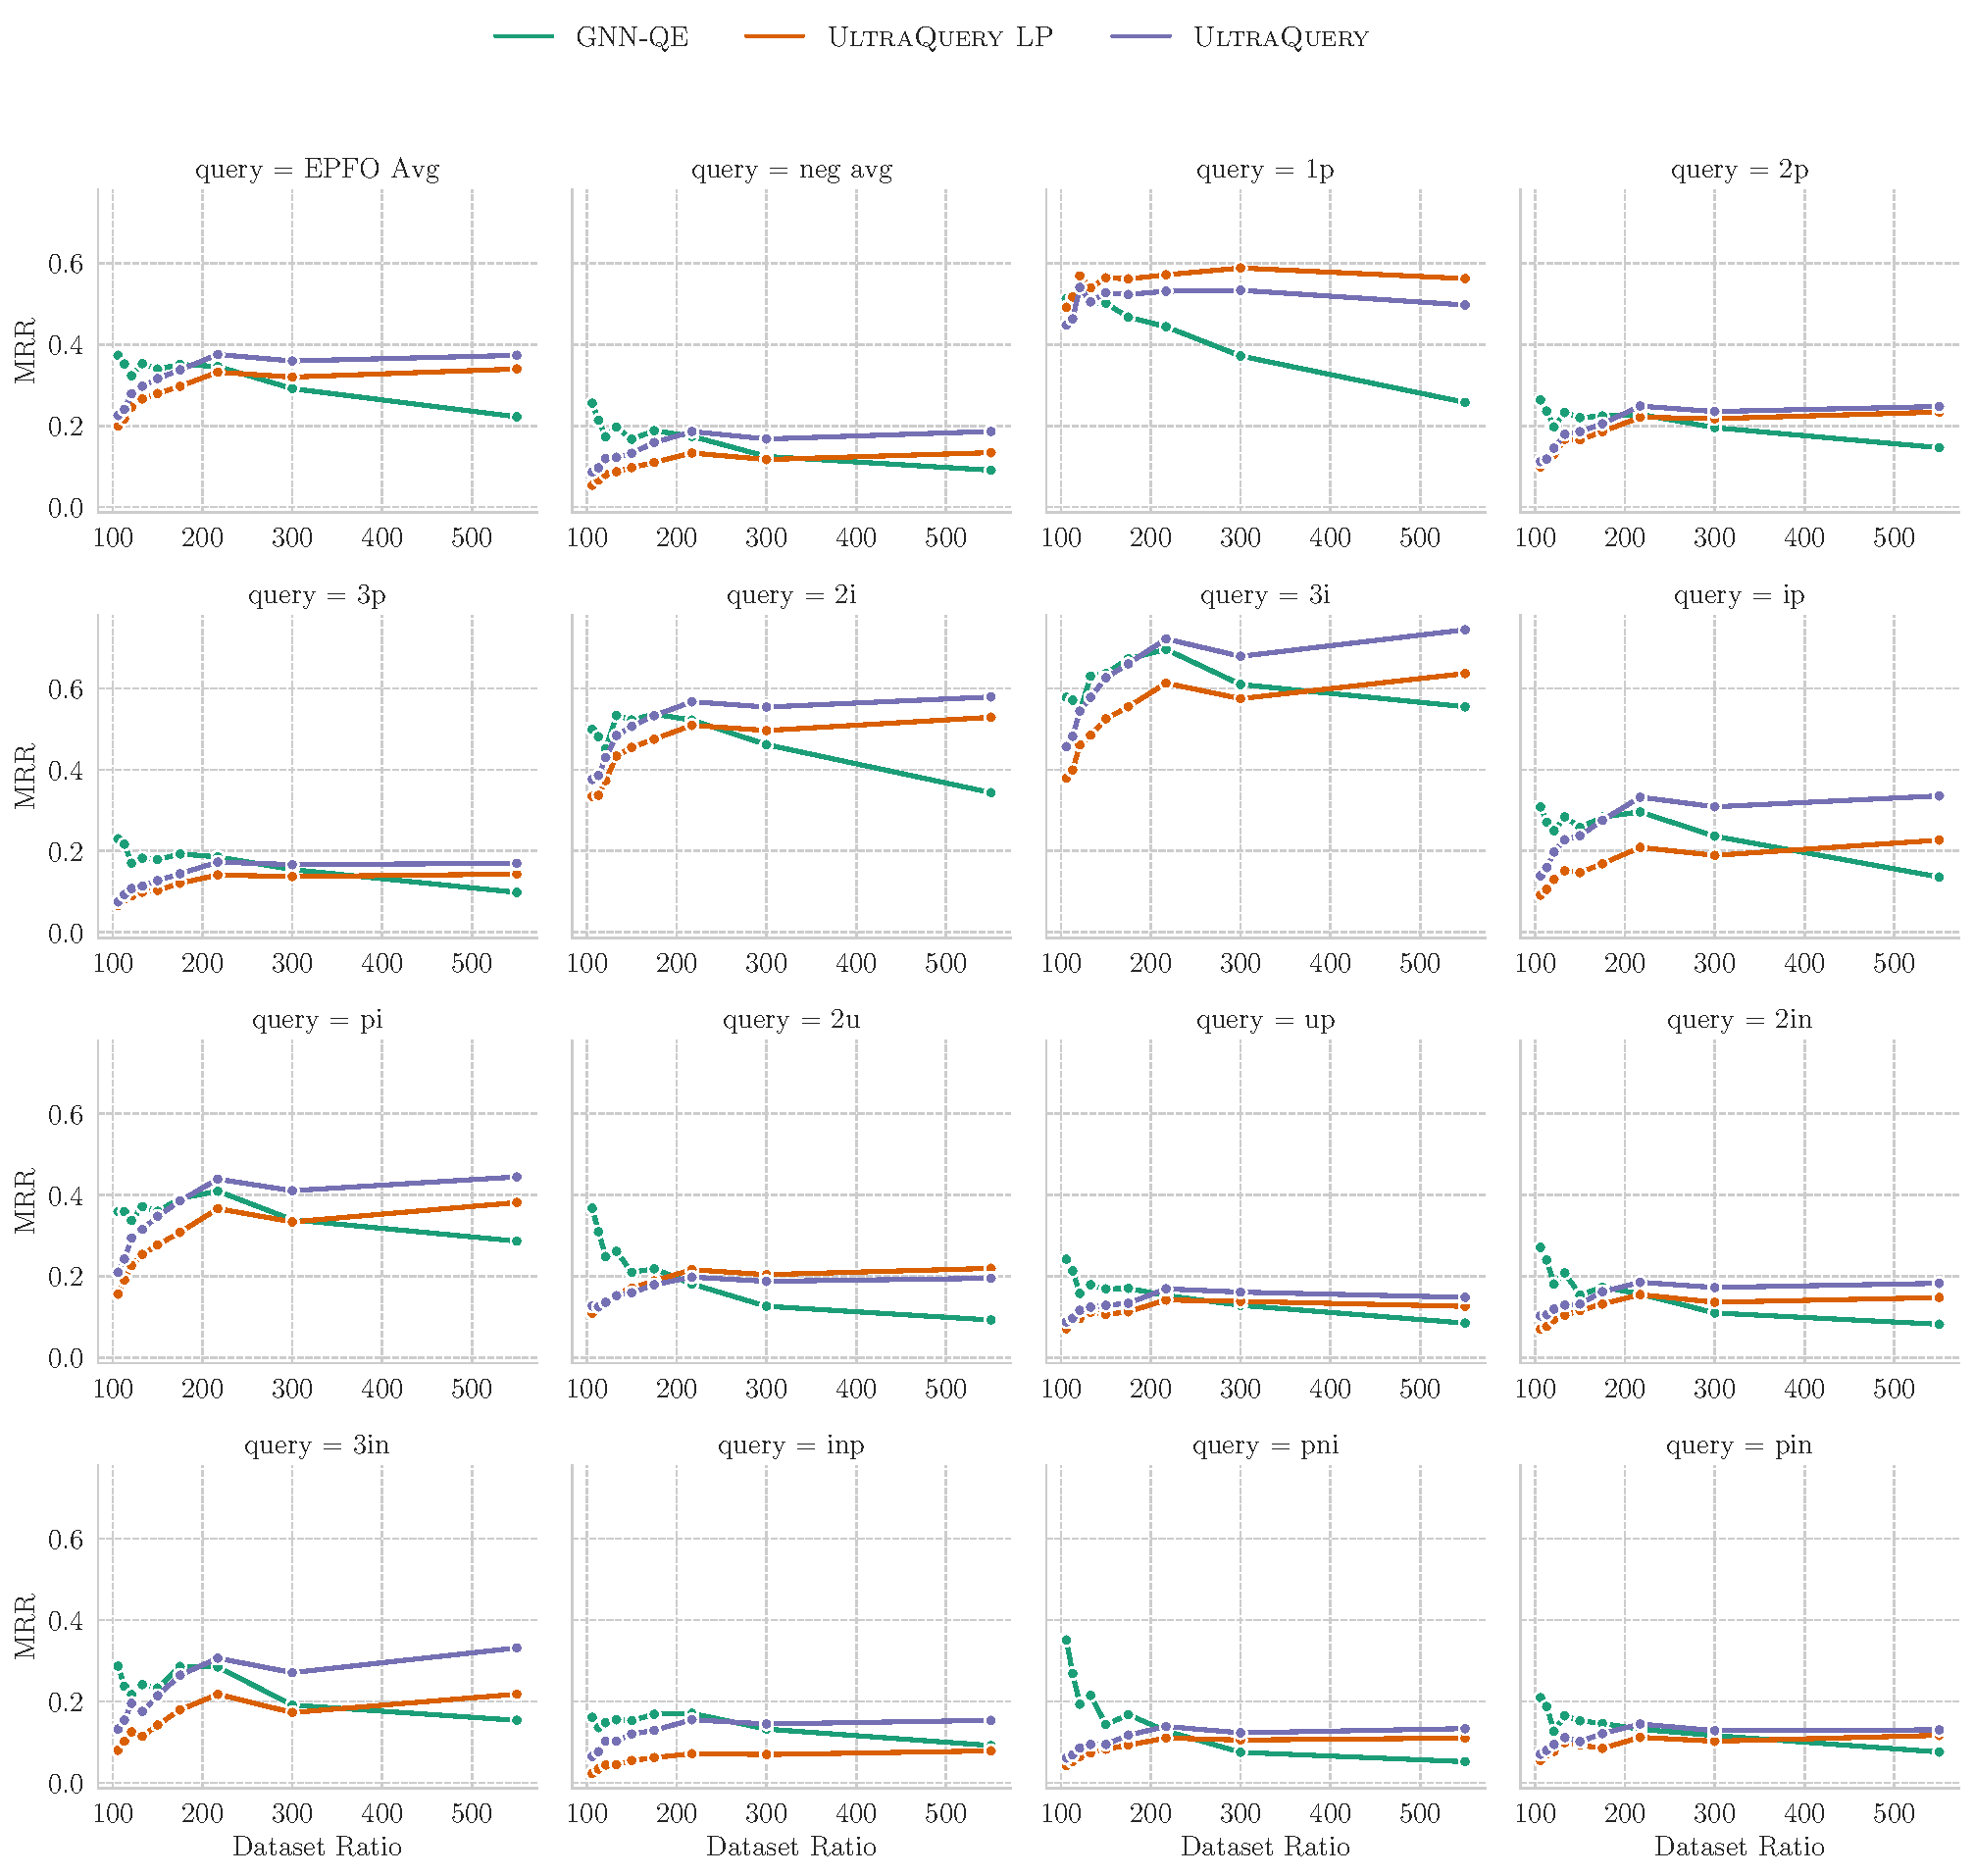
\includegraphics[width=\linewidth]{figs/app_inde_pyg.pdf}
    \caption{Full results on 9 inductive $(e)$ datasets corresponding to \autoref{fig:abl_multisource}: albeit \methodlp outperforms the main \method on simple \emph{1p} queries, it suffers from the multi-source propagation issue on complex queries. \method trades a fraction of 1p query performance for significantly better average performance on 9 EPFO and 5 negation query types with particularly noticeable gains on intersection and \emph{2in}, \emph{3in} queries. }
    \label{fig:app_inde_full}
\end{figure*}


%%%% Multi-source propagation issue %%%
% \section{More Analysis on Multi-Source Propagation Issue}
